\documentclass[preprint]{elsarticle}
%\documentclass[review,number,sort&compress]{elsarticle}

\usepackage{amssymb}
\usepackage{amsmath}
\usepackage{graphicx}
\usepackage[load-configurations=abbreviations]{siunitx}
\usepackage[european]{circuitikz}
\usepackage{xstring}
\usepackage{tikz}
\usepackage{verbatim}
\usepackage[active]{srcltx}
\usepackage{multicol}
%\usepackage{lipsum}
\usepackage{graphicx}
\usepackage{nicefrac}
\usepackage{fancyhdr}
\usepackage[english]{babel}
\usepackage{color}
%% The amsthm package provides extended theorem environments
%% \usepackage{amsthm}
\newcommand{\sigmabin}{\ensuremath{\mathnormal{\sigma_{\textrm{bin}}}}}
\newcommand{\sigmaimp}{\ensuremath{\mathnormal{\sigma_{\textrm{imp}}}}}
\newcommand{\deltaimp}{\ensuremath{\mathnormal{\delta_{\textrm{imp}}}}}

\newcommand{\Allpixsquared}{\ensuremath{\textrm{AllPix}^{2}}}
%\newcommand{\Allpixsquared}{\ensuremath{\textrm{AllPix}}}

\newcommand{\vect}[1]{\boldsymbol{#1}}

%% The lineno packages adds line numbers. Start line numbering with
%% \begin{linenumbers}, end it with \end{linenumbers}. Or switch it on
%% for the whole article with \linenumbers after \end{frontmatter}.
\usepackage{lineno}


%linenumbers
\setpagewiselinenumbers
\modulolinenumbers[5]

\begin{document}

\begin{frontmatter}


\title{Simulation of enhanced lateral drift sensors}

\author[desy]{A.~Velyka}
\ead{anastasiia.velyka@desy.de}
\address[desy]{Notkestr. 85, 22607 Hamburg, Germany}

\author[cern]{S.~Spannagel}
\ead{simon.spannagel@cern.ch}
\address[cern]{Route de , Geneva, Switzerland}

\author[desy]{H.~Jansen\corref{cor1}}
\ead{hendrik.jansen@desy.de}

\cortext[cor1]{Corresponding author}


\begin{abstract}
We propose a novel concept of a layer-wise produced semiconductor sensor for precise charged particle tracking called Enhanced Lateral Drift (ELAD) sensor. 
In ELAD sensors the spatial resolution of the impact position of ionising particles is improved by a dedicated charge sharing mechanism,
 which is achieved by a non-homogeneous electric field in the lateral direction in the sensor bulk. 
The non-homogeneous electric field is created by buried doping implants with a higher concentration with respect to the background concentration of the bulk. 
The resulting position-dependent charge sharing allows for an improved interpolation of the impact position. 

TCAD-based electric field simulations for 2D and 3D geometries as well as transient simulations with a traversing particle for the 2D geometry have been carried out.
The electric field profiles have further been optimised for position resolution making use of the $\Allpixsquared$ detector simulation framework.
The simulations show a strong dependence of the charge sharing mechanism on the buried implant concentration.
Optimal values for the buried implant concentration allow for nearly linear charge sharing between two readout electrodes as a function of the impact position.
In-depth studies of the detector performance reveal achievable RMS position resolution of XX for a 150\,um tick and XX um for a 50 um thick sensor using a 55 um pitch. 
Additionally, the foreseen production technique combining silicon epitaxy and ion beam implantation is outlined.
\end{abstract}

\begin{keyword}
Semiconductor detector \sep deep bulk engineering \sep conceptual design \sep precision particle tracking
\PACS 29.40.Wk \sep 72.20.Fr
\end{keyword}

\end{frontmatter}

\linenumbers
\section{Introduction}
% Precision measurements of Higgs decays at a future collider necessitate charged particle detectors with single point resolutions of about $\SI{3}{\um}$ at sensor thickness at or below $\SI{100}{\um}$.~\cite{DominiksCLICNote}
% These requirements drive the mainstream  of detector R\&D for collider experiments towards smaller and smaller sensor unit-cells, or pitches.
% However, this evolutionary approach increases the number of read-out channels resulting in various disadvantages. 
% In this work, a new sensor concept is presented that exemplifies a strategy towards achieving the theoretical optimum of position resolution. 
% It avoids the small pitch paradigm as much as possible and renders optimal spatial resolution possible, even at sensor thicknesses of the order of $\SI{50}{\um}$.
% In this new approach, implants (volumes with higher doping concentration compared to the background concentration) deep inside the bulk of the sensor
%  guide the charge cloud produced by a traversing particle laterally towards the boarder between two unit-cells, thus enhancing charge sharing between neighbouring strips/pixels. 
% With appropriately placed deep implants, the lateral drift can be optimised towards an optimal, i.e.\ linear charge sharing and hence optimal resolution of the incident position at a given pitch size. 
% In this concept of an enhanced lateral drift (ELAD) sensor,
%  the degree of linearity of the charge sharing and Landau fluctuations of the energy loss along the particle  trajectory limit the sensor resolution. %FIXME check if this is true :D
%  
% This is some reference that can be deleted~\cite{Moliere:1948zz,PhysRev.89.1256}

Experiments at possible future colliders like CLIC\footnote{Compact Linear Collider}~\cite{cdr} and ILC\footnote{International Linear Collider}~\cite{ILCcdr} aim, among others,
 for a precise measurement of Higgs decays to pairs of b-quarks, c-quarks and gluons and efficient identification of top quarks in the decay t$\mathrm{\rightarrow}$Wb.
To this end, the experiments require light-weight detectors with a single-point resolution of a few micrometers. 
E.g., the tracker and vertex detectors for CLIC require a single point resolution of better than $\SI{7}{\um}$ and $\SI{3}{\um}$, respectively, in the transverse plane
 to meet the requirements on the track-momentum and impact parameter resolution at a total silicon detector thickness of less than $\SI{100}{\um}$~\cite{det}.
Several options for tracking and vertex sensor technology are considered for CLIC, among them are monolithic and hybrid detectors~\cite{clicyellowreport}.

This work focuses on a new type of a hybrid detector aiming to meet the requirements of the CLIC vertex detector.
A common approach to achieve an improved position resolution in silicon detectors is to decrease the readout cell size.
This leads to an increased number of readout channels and less area for logic per channel on the readout chip.
Additionally, the miniaturisation of interconnection techniques might present limits. 

The position resolution can also be improved by means of charge sharing, i.e.\ by collecting the charge on more than one readout electrode.
Geometric charge sharing is used e.g.\ in the CMS experiment by tilting the sensors in the Endcap~\cite{simon}. 
Lorentz drift induced charge sharing by means of a magnetic field is realised in the barrel section of the experiment~\cite{cmstdr}.
However, these two methods do not provide sufficient charge sharing in thin ($\leq \SI{100}{\um}$) sensors~\cite{clicyellowreport},
 as either unrealistically strong magnetic fields or huge sensor tilts would be necessary, the latter in turn increasing the material budget.

The hybrid detector proposed herein, a so-called Enhanced Lateral Drift (ELAD) sensor in combination with a readout ASIC,
 introduces a lateral electric field component in the sensor bulk yielding a lateral charge drift to achieve a position resolution of a few micrometre. 
This lateral component of the electric field is created by regions deep within the sensor bulk featuring a higher doping concentration with respect to the background doping concentration.
This diminishes the need to downsize the sensor pitch while avoiding sensor tilt or magnetic fields. 

In Sec.~\ref{sec:con}, we detail the concept of the ELAD sensor.
ADD MORE


\section{The concept of ELAD sensors}
\label{sec:con}
Charged particles traversing a silicon sensor create free electron-hole pairs, which drift inside the sensor following the electric field lines.
Due to insufficient diffusion in thin, depleted, standard planar sensors the created charge is collected almost entirely by the nearest electrode and only a small fraction of it by the neighbouring electrode.
Therefore, in this particular case, an improved position resolution is solely achieved by downsizing the strip/pixel pitch.

\begin{figure}[t]
  \centering
  \includegraphics[height=4.1cm]{figures/concept4.pdf}\put(-269, 115){RO}\put(-225, 125){\footnotesize unit cell}\put(-227.5, 117){\footnotesize boundary}\put(-165, 115){RO}\put(-120, 125){\footnotesize unit cell}\put(-122.5, 117){\footnotesize boundary}\put(-61, 115){RO}\put(-215, 50){\rotatebox{90}{\small diffusion}}\put(-110, 50){\rotatebox{90}{\small diffusion}}
  \caption{
A sketch of the charge sharing mechanism in ELAD sensors is shown. 
Arrows indicate the direction of the field strength. 
}
  \label{fig:concept}
\end{figure}

The concept of the ELAD sensor is based on a dedicated charge sharing mechanism independent of sensor tilt and magnetic fields.
Local modifications to the electric field yield a position-dependent charge collection at two electrodes~\cite{hj}.
To this end, the electric field profile is altered by buried implants with higher doping concentration with respect to the background doping concentration of the bulk. 
The buried implants are arranged in layers forming a trapezoidal area changing the electric field lines in such a way
 that the charge carriers, e.g.\ holes in an n-type sensor, drift towards the centre between two electrodes to possibly diffuse into the next unit cell, see Fig.~\ref{fig:concept}.
This scheme results in a partial collection at two electrodes.
An optimal position resolution is achieved if the distribution of the collected charge between two electrodes is a linear function of the particle's impact position, 
 i.e.\ the entirety of the charge is collected at one electrode if the impact position is in the centre of the readout electrode,
 the charge is equally shared between two electrodes if the impact position is half-way between two electrodes
 and in between the shared fraction of the charge increases linearly with the distance to the electrode's centre.
Our realisation of an ELAD sensor contains two types of buried implants: p-implants and n-implants, effectively reducing the impact of the additional stationary charges on $N\mathrm{_{eff}}$~\cite{elad}. 
With such a balancing of p- and n-implants, a similar depletion voltage as in a standard planar sensor with an epitaxial layer of the same background concentration and thickness is achieved.
The utilisation of two types of buried implants also creates a stronger electric field in the lateral direction, thereby improving the charge-sharing behaviour.

\section{Device optimisation of an ELAD sensor}

Initial geometry, optimisation strategy, static and transient, ...

E-fields, tcad eta functions

\section{Monte Carlo studies}

AP2, which modules, settings, manipulations of the TCAD field (2D to 3D), MIPs, drift and diff, 

AP2 eta functions, residuals

\section{Discussion}

single point res a.f.o various parameters: concentration, bias voltage, thickness, maybe turn on/off Landau if possible

'thoughts on production'

\begin{figure}[t]
  \centering
  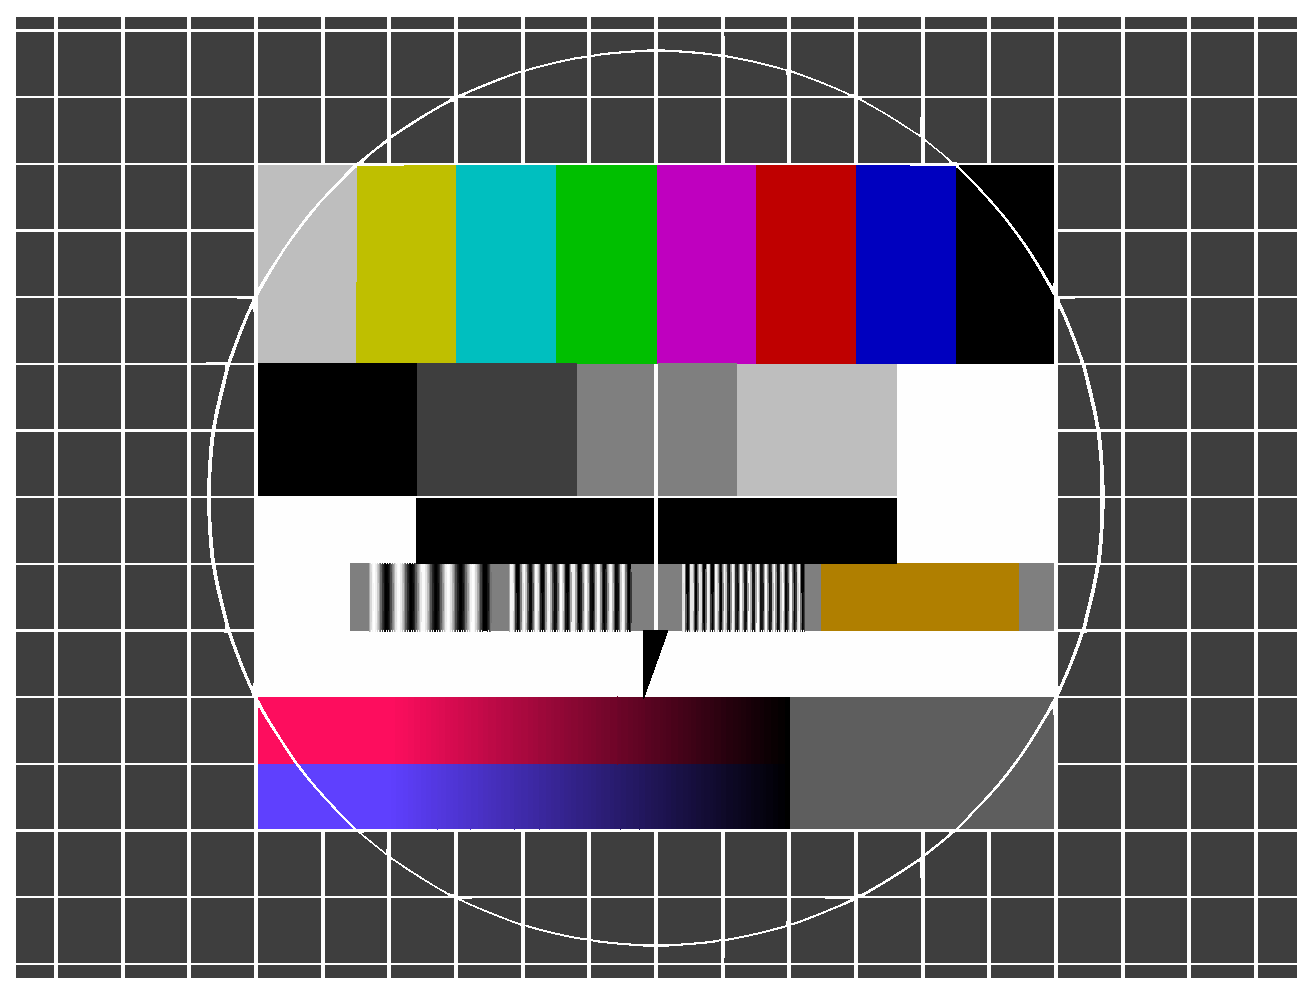
\includegraphics[width=0.8\textwidth]{figures/testcard} %\put(-35,0){$[\si{\um}]$} \put(-335,180){$[\si{\um}]$}
  \caption{dummy}
\label{fig:dummy}
\end{figure}

\section{Conclusion}


\section*{Acknowledgement}
This project is funded via the DESY Strategy Funds.

\small
\section*{References}
\bibliographystyle{unsrt}
\bibliography{bibtex/refs}


\end{document}
